\documentclass[border=6pt]{standalone}
% Shared typography and colours for the standalone figures.
\usepackage{unicode-math}
\setmainfont{TeX Gyre Heros}
\setmathfont{TeX Gyre Pagella Math}
\usepackage{tikz}
\usetikzlibrary{arrows.meta,positioning,calc,decorations.pathreplacing}
\usepackage{pgfplots}
\pgfplotsset{compat=1.18}

% One colour per element or subsystem. Record the mapping in
% the working repository conventions and use it identically in every figure.
\definecolor{elemA}{HTML}{1F5FA8}
\definecolor{elemB}{HTML}{B8461B}
\definecolor{elemC}{HTML}{2E7D32}
\definecolor{elemD}{HTML}{6A4C93}
\definecolor{frameline}{HTML}{555555}

\begin{document}
\hyphenpenalty=10000
\exhyphenpenalty=10000
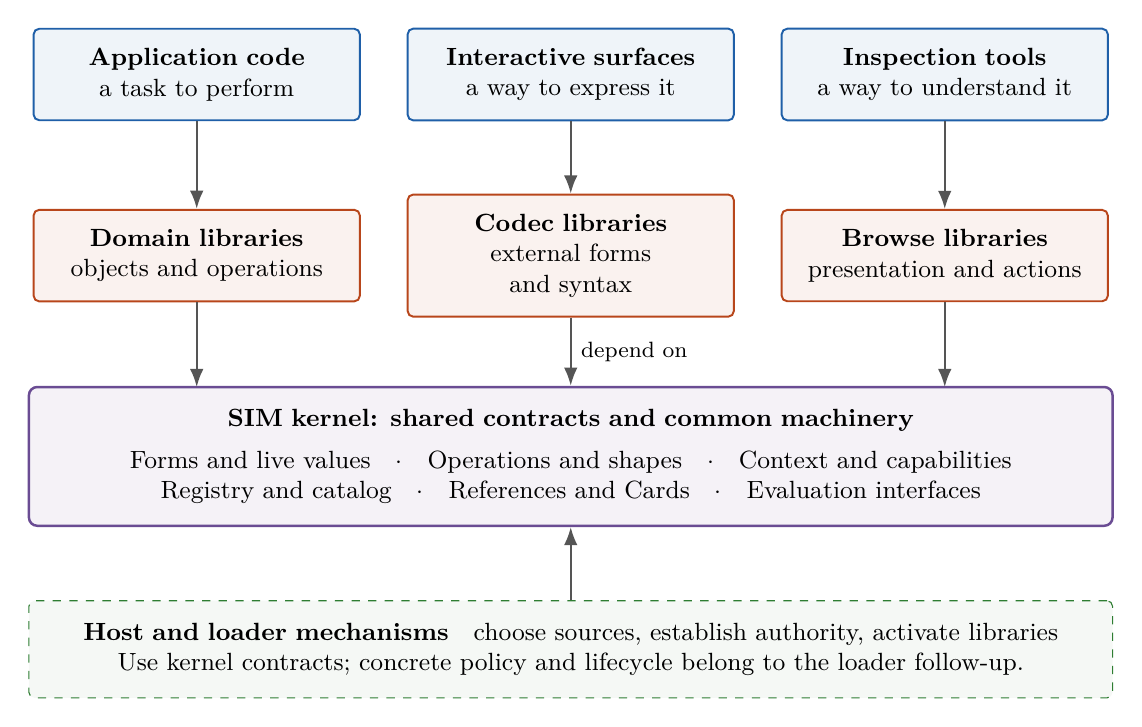
\begin{tikzpicture}[font=\small,
box/.style={draw=#1,fill=#1!7,rounded corners=2pt,line width=.7pt,text width=3.65cm,minimum height=1.15cm,align=center,inner sep=7pt},
arrow/.style={-{Latex[length=2.3mm]},line width=.8pt,draw=frameline}]
\node[box=elemA] (app) at (-4.75,4.8) {\textbf{Application code}\\a task to perform};
\node[box=elemA] (human) at (0,4.8) {\textbf{Interactive surfaces}\\a way to express it};
\node[box=elemA] (tool) at (4.75,4.8) {\textbf{Inspection tools}\\a way to understand it};
\node[box=elemB] (domain) at (-4.75,2.5) {\textbf{Domain libraries}\\objects and operations};
\node[box=elemB] (codec) at (0,2.5) {\textbf{Codec libraries}\\external forms and syntax};
\node[box=elemB] (browse) at (4.75,2.5) {\textbf{Browse libraries}\\presentation and actions};
\draw[arrow] (app)--(domain);
\draw[arrow] (human)--(codec);
\draw[arrow] (tool)--(browse);
\node[draw=elemD,fill=elemD!7,rounded corners=3pt,line width=.9pt,
 text width=13.2cm,minimum height=1.6cm,align=center,inner sep=8pt] (kernel) at (0,-.05)
 {\textbf{SIM kernel: shared contracts and common machinery}\\[4pt]
 Forms and live values\quad $\cdot$\quad Operations and shapes\quad $\cdot$\quad Context and capabilities\\
 Registry and catalog\quad $\cdot$\quad References and Cards\quad $\cdot$\quad Evaluation interfaces};
\draw[arrow] (domain.south)--(-4.75,.83);
\draw[arrow] (codec.south)--node[right,font=\footnotesize]{depend on}(kernel.north);
\draw[arrow] (browse.south)--(4.75,.83);
\node[draw=elemC,dashed,fill=elemC!5,rounded corners=2pt,text width=13.2cm,
 align=center,inner sep=8pt] (host) at (0,-2.5)
 {\textbf{Host and loader mechanisms}\quad choose sources, establish authority, activate libraries\\
 Use kernel contracts; concrete policy and lifecycle belong to the loader follow-up.};
\draw[arrow] (host.north)--(kernel.south);
\end{tikzpicture}
\end{document}
